\documentclass[11pt]{article}

\usepackage{times}
\usepackage{epsf}
\usepackage{epsfig}
\usepackage{amsmath, alltt, amssymb, xspace}
\usepackage{wrapfig}
\usepackage{fancyhdr}
\usepackage{url}
\usepackage{verbatim}
\usepackage{fancyvrb}

\usepackage{subfigure}
\usepackage{cite}
\usepackage{hyperref}
\hypersetup{%
    pdfborder = {0 0 0}
}
%\usepackage{cases}
%\usepackage{ltexpprt}
%\usepackage{verbatim}

%\topmargin      -0.70in  % distance to headers
%\headheight     0.2in   % height of header box
%\headsep        0.4in   % distance to top line
%\footskip       0.3in   % distance from bottom line

% Horizontal alignment
\topmargin      -0.50in  % distance to headers
\oddsidemargin  0.0in
\evensidemargin 0.0in
\textwidth      6.5in
\textheight     8.9in 


%\centerfigcaptionstrue

%\def\baselinestretch{0.95}


\newcommand\discuss[1]{\{\textbf{Discuss:} \textit{#1}\}}
%\newcommand\todo[1]{\vspace{0.1in}\{\textbf{Todo:} \textit{#1}\}\vspace{0.1in}}
\newtheorem{problem}{Problem}[section]
%\newtheorem{theorem}{Theorem}
%\newtheorem{fact}{Fact}
\newtheorem{define}{Definition}[section]
%\newtheorem{analysis}{Analysis}
\newcommand\vspacenoindent{\vspace{0.1in} \noindent}

%\newenvironment{proof}{\noindent {\bf Proof}.}{\hspace*{\fill}~\mbox{\rule[0pt]{1.3ex}{1.3ex}}}
%\newcommand\todo[1]{\vspace{0.1in}\{\textbf{Todo:} \textit{#1}\}\vspace{0.1in}}

%\newcommand\reducespace{\vspace{-0.1in}}
% reduce the space between lines
%\def\baselinestretch{0.95}

\newcommand{\fixmefn}[1]{ \footnote{\sf\ \ \fbox{FIXME} #1} }
\newcommand{\todo}[1]{
\vspace{0.1in}
\fbox{\parbox{6in}{TODO: #1}}
\vspace{0.1in}
}

\newcommand{\mybox}[1]{
\vspace{0.2in}
\noindent
\fbox{\parbox{6.5in}{#1}}
\vspace{0.1in}
}


\newcounter{question}
\setcounter{question}{1}

\newcommand{\myquestion} {{\vspace{0.1in} \noindent \bf Question \arabic{question}:} \addtocounter{question}{1} \,}

\newcommand{\myproblem} {{\noindent \bf Problem \arabic{question}:} \addtocounter{question}{1} \,}



\newcommand{\copyrightnotice}[1]{
\vspace{0.1in}
\fbox{\parbox{6in}{\small Copyright \copyright\ 2014\ \ Wenliang Du, Syracuse University.\\
      The development of this document is/was funded by the following grants from
      the US National Science Foundation: No. 1303306 and 1318814.
      This lab was altered and imported into the Labtainer framework by the Naval Postgraduate
      School, Center for Cybersecurity and Cyber Operations under National Science
      Foundation Award No. 1438893.
      Permission is granted to copy, distribute and/or modify this document
      under the terms of the GNU Free Documentation License, Version 1.2
      or any later version published by the Free Software Foundation.
      A copy of the license can be found at http://www.gnu.org/licenses/fdl.html.}}
\vspace{0.1in}
}

\newcommand{\copyrightnoticeA}[1]{
\vspace{0.1in}
\fbox{\parbox{6in}{\small Copyright \copyright\ 2006\ \ Wenliang Du, Syracuse University.\\
      The development of this document was partially funded by
      the National Science Foundation's Course, Curriculum, and Laboratory
      Improvement (CCLI) program under Award No. 0618680 and 0231122.
      This lab was altered and imported into the Labtainer framework by the Naval Postgraduate
      School, Center for Cybersecurity and Cyber Operations under National Science
      Foundation Aware No. 1438893.

      Permission is granted to copy, distribute and/or modify this document
      under the terms of the GNU Free Documentation License, Version 1.2
      or any later version published by the Free Software Foundation.
      A copy of the license can be found at http://www.gnu.org/licenses/fdl.html.}}
\vspace{0.1in}
}


\newcommand{\nocopyrightnotice}[1]{
\vspace{0.1in}
\fbox{\parbox{6in}{\small  
      The development of this document is funded by 
      the National Science Foundation's Course, Curriculum, and Laboratory 
      Improvement (CCLI) program under Award No. 0618680 and 0231122. 
      Permission is granted to copy, distribute and/or modify this document.
      }}
\vspace{0.1in}
}

\newcommand{\idea}[1]{
\vspace{0.1in}
{\sf IDEA:\ \ \fbox{\parbox{5in}{#1}}}
\vspace{0.1in}
}

\newcommand{\questionblock}[1]{
\vspace{0.1in}
\fbox{\parbox{6in}{#1}}
\vspace{0.1in}
}


\newcommand{\minix}{{\tt Minix}\xspace}
\newcommand{\unix}{{\tt Unix}\xspace}
\newcommand{\linux}{{\tt Linux}\xspace}
\newcommand{\ubuntu}{{\tt Ubuntu}\xspace}
\newcommand{\selinux}{{\tt SELinux}\xspace}
\newcommand{\freebsd}{{\tt FreeBSD}\xspace}
\newcommand{\solaris}{{\tt Solaris}\xspace}
\newcommand{\windowsnt}{{\tt Windows NT}\xspace}
\newcommand{\setuid}{{\tt Set-UID}\xspace}
%\newcommand{\smx}{{\tt Smx}\xspace}
\newcommand{\smx}{{\tt Minix}\xspace}
\newcommand{\relay}{{\tt relay}\xspace}
\newcommand{\isys}{{\tt iSYS}\xspace}
\newcommand{\ilan}{{\tt iLAN}\xspace}
\newcommand{\iSYS}{{\tt iSYS}\xspace}
\newcommand{\iLAN}{{\tt iLAN}\xspace}
\newcommand{\iLANs}{{\tt iLAN}s\xspace}
\newcommand{\bochs}{{\tt Bochs}\xspace}

\newcommand\FF{{\mathcal{F}}}

\newcommand{\argmax}[1]{
\begin{minipage}[t]{1.25cm}\parskip-1ex\begin{center}
argmax
#1
\end{center}\end{minipage}
\;
}

\newcommand{\bm}{\boldmath}
\newcommand  {\bx}    {\mbox{\boldmath $x$}}
\newcommand  {\by}    {\mbox{\boldmath $y$}}
\newcommand  {\br}    {\mbox{\boldmath $r$}}


%\pagestyle{fancyplain}
%\lhead[\thepage]{\thesection}      % Note the different brackets!
%\rhead[\thesection]{SEED Laboratories}
%\lfoot[\fancyplain{}{}]{Syracuse University} 
%\cfoot[\fancyplain{}{}]{\thepage} 

\newcommand{\tstamp}{\today}   
%\lhead[\fancyplain{}{\thepage}]         {\fancyplain{}{\rightmark}}
%\chead[\fancyplain{}{}]                 {\fancyplain{}{}}
%\rhead[\fancyplain{}{\rightmark}]       {\fancyplain{}{\thepage}}
%\lfoot[\fancyplain{}{}]                 {\fancyplain{\tstamp}{\tstamp}}
%\cfoot[\fancyplain{\thepage}{}]         {\fancyplain{\thepage}{}}
%\rfoot[\fancyplain{\tstamp} {\tstamp}]  {\fancyplain{}{}}

\pagestyle{fancy}
%\lhead{\bfseries Computer Security Course Project}
\lhead{\bfseries SEED Labs}
\chead{}
\rhead{\small \thepage}
\lfoot{}
\cfoot{}
\rfoot{}




\begin{document}

\begin{center}
{\LARGE PLC and Modbus}
\vspace{0.1in}\\
\end{center}


\section{Overview}
This exercise explores the use of the Modbus protocol and a
PLC to control a simple device.
It is assumed the student has had an introduction to PLC's, ladder logic and 
the Modbus protocol.  It is also assumed the student has some experience with
Wireshark.

Details of the Modbus protocol can be found at:
\url {https://http://modbus.org/docs/PI\_MBUS\_300.pdf}
A tutorial on the use of Ladder Logic is at:
\url {//https://www.plcacademy.com/ladder-logic-tutorial/}


\section{Lab Environment}
This lab runs in the Labtainer framework,
available at http://my.nps.edu/web/c3o/labtainers.
That site includes links to a pre-built virtual machine
that has Labtainers installed, however Labtainers can
be run on any Linux host that supports Docker containers.

From your labtainer-student directory start the lab using:
\begin{verbatim}
    labtainer softplc2
\end{verbatim}
Links to this lab manual will be displayed.  

\section{Lab topology}
The lab includes three components as shown in \ref{topology}:
\begin{itemize}
\item{Slave Device} A simple slave device containing two buttons and a lamp.  The device has an
ethernet interface via which it is connected to a PLC using Modbus TCP/IP.
\item{PLC} A programable logic controller implemented using the OpenPLC Soft-PLC implementation
on a Linux based computer.  The PLC is connected to the slave device via Modbus TCP/IP over ethernet.
The PLC has a seperate ethernet connection to an HMI computer.
For convenience of the lab, the PLC computer includes Wireshark and will be used to capture, review and
replay network traffic between the PLC and the slave device.  

\item{HMI} A computer that interacts with the PLC using a web browser to load programs and monitor its operation.  This
computer also contains an OpenPLC Editor for constructing programs using ``Ladder Logic'' (LD).
\end{itemize}

The PLC and the slave device communicate via Modbus TCP/IP, with the PLC acting as the master.  
The HMI component in this topology does not use Modbus, rather it simply interacts with the PLC via the
PLC's web server.
\begin{figure}[H]
\begin{center}
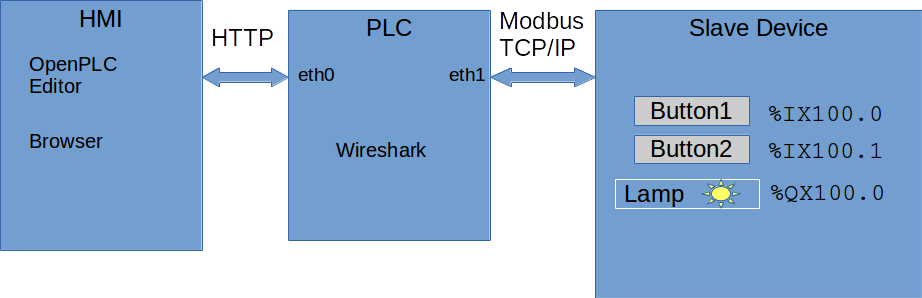
\includegraphics [width=0.8\linewidth]{softplc2.png}
\end{center}
\caption{Soft PLC Lab Topology}
\label{fig:topology}
\end{figure}

\section{Tasks}
In this lab, you will create a simple ``hello world'' Structured Text program using Ladder Logic.  You will upload this program
from the HMI to the PLC and use it to control the slave device.  You will use Wireshark to observe traffic between
the PLC and the slave device.

\subsection{Explore}
Find the {\tt Physical Board} window.  This is your virtual slave device.  Click the two buttons and confirm nothing happens.
This board is connected to the PLC via Modbus TCP/IP, however the PLC is not yet running and is not yet programmed.

\subsection{Build and run PLC program}
In this task, you will deploy an existing ``hello world'' program onto the PLC and demonstrate its use.
\subsubsection{Build the Hello World Program}
On the HMI window, start the OpenPLC Editor in the background:
\begin{verbatim}
    OpenPLC_Editor/openplc_editor.sh &
\end{verbatim}
\begin{figure}[H]
\begin{center}
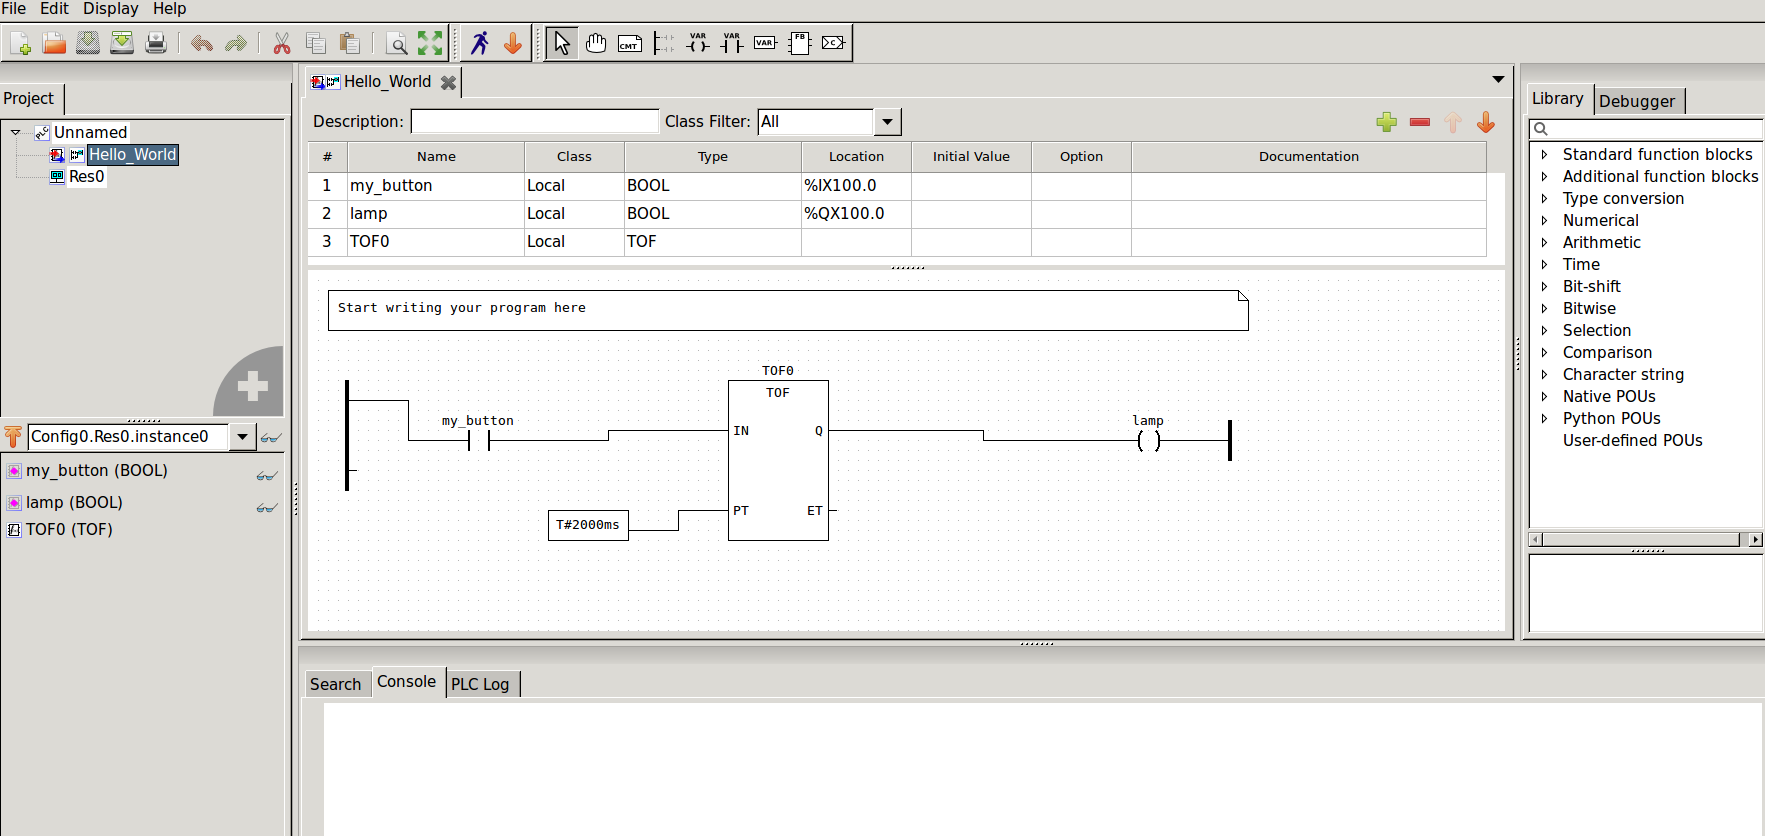
\includegraphics [width=0.8\linewidth]{openplcEditor.png}
\end{center}
\caption{OpenPLC Editor}
\label{fig:editor}
\end{figure}

When the editor window displays, use {\tt File / Open} and select {\tt hello}.  Then double-click on the
{\tt Hello World} entry in the project pane on the upper left of the window.  This is an example of a LD program that 
states that if the button is pushed, then the lamp should be lit and remain on for 2 seconds after the button is
released.  

Use the orange down arrow on the menu bar to generate the program for the OpenPLC runtime.  When prompted, save the 
file in a file with a {\tt .st} file extension.  Make a note of the directory where you saved the file.  This operation
has converted the LD program into a Structured Text (ST) program, which is form that OpenPLC works with.

You may now close or minimize the OpenPLC Editor.  Back on the HMI terminal, find the ST file that you saved 
and display its contents.  That is the program the PLC will run in order to control the slave device.  As you can see,
ST programs have recognizable programming constructs.  You will be asked to modify this program later.

\subsection{Start the PLC user interface \& Explore}
On the HMI terminal, use the firefox browser to access the PLC using port 8080:
\begin{verbatim}
    firefox plc:8080 &
\end{verbatim}
\noindent Login to the PLC through the browser with {\tt openplc} as the username and password.  
You should now see the Open PLC web page that controls the PLC.  Click the {\tt Slave Devices} button
on the left.  And double click on the {\tt myserver entry}.  This is the slave device that your PLC program will control.
Note we define only 3 bits to control the slave device.  Two bits as \textit{Descrete Inputs} for two buttons (only one 
of which is initially used), an one bit for the lamp as \textit{Coils}.
Make a note of the slave device IP address and  the port number used to communicate using Modbus.

\subsubsection{Upload the ST program to the PLC}
Select {\tt Programs} on the left pane and use the
{\tt Browse} button to locate your ST file.  Then upload it to the PLC.  Provide a {\tt Name} in the resulting form
and press the {\tt Upload program} button.  Note the program is compiled on the PLC and results are displayed in
the browser.  Then click the {\tt Go to Dashboard} button.

The PLC now has your {\tt hello world} program loaded, but the PLC is not yet running.
Click the {\tt Start PLC} button.  Once the PLC is started, click the Monitoring button.

\subsubsection{Test the PLC program}
On the Physical Board, click button1.  The light bulb should come on for a few seconds.  Observe the indicators on the browser
Monitoring page.  

\subsection{Observe Modbus traffic}
The PLC component includes Wireshark for monitoring the PLC network traffic.
Find the {\tt plc} window, and start wireshark:
\begin{verbatim}
wireshark &
\end{verbatim}
\noindent Review the Modbus traffic.  Note that Wireshark automatically detects the Modbus traffic, and displays the protocol.
Note how all of the Modbus exchanges are either queries from the PLC or responses from the slave.
Click {\tt button1}.  Then stop the Wirshark capture (red square button on the menu). 

Locate a packet that directed the lamp to light.  Note using a display filter of {\tt modbus.data==1} will filter the 
packets to include only queries that set the coil (lamp) to on, and responses that reflect the button is pressed.
Once you've identified and selected the packet, click on the {\tt Modbus/TCP} field and save the raw bytes to a file named
{\tt on.raw} using {\tt File / Export Packet Bytes}.  

Then locate a packet that directed the lamp to turn off.  Save its {\tt Modbus/TCP} raw bytes to a file named {\tt off.raw}.

\subsection{Replay coil commands}
Stop the PLC if it is running (click the {\tt Stop PLC} button in the browser).
In the plc window, locate the files you just saved.  Then use netcat to replay them to the slave device.
\begin{verbatim}
cat on.raw | nc <ip> <port>
cat off.raw | nc <ip> <port>
\end{verbatim}
\noindent Where ip and port are the IP address and port of the slave device.
Note that the capturing and replaying of TCP packets is performed on the PLC computer for convenience of the lab.  
It could occur on any component with access to the network used by the PLC to communicate with the slave device.

\subsection{Modify the ST program}
Stop the PLC if it is running (click the {\tt Stop PLC} button in the browser).
Go to the HMI terminal.  
Edit your ST file and change the delay from 2000 ms to 10,000 ms.
Back on the browser, go to programs and upload the ST file again, this time giving the program a different name.
Start the PLC and click button1.  Confirm that your program change has modified the PLC operation.

\subsection{Modify the LD program}
Stop the PLC and go back to the HMI terminal and return to the OpenPLC editor.  Use the editor to define a second button
such that pressing either button will cause the lamp to light. You may wish to first use {\tt File / Save As / Create Folder} 
to create a copy of the hello world program.  To edit the LD program:
\begin{itemize}
\item{Add button to table} Click {\tt my\_button} field in the table and then click the green {\tt +} icon to add 
a row to the table of items. Change the name of the new item to {\tt my\_button2}.  Note the editor has assigned the very next
{\tt Location} value, which is what we want.
\item{Add button to schematic} Click the {\tt contact} icon in the menu and then click on the diagram where the new button is to go.
Assign {\tt my\_button2} as the variable name.
\item{Connect button} Click on the unused lead of the power rail and drag a line to the left lead of the button.  Then click the 
right lead of the button and drag a line to the {\tt In} pin of the {\tt TOF0} (Timer Off-Delay) component.
\end{itemize}
Then save your changes and use the orange down arrow to generate a new ST file and save it.
Load your new program into the PLC and run it.  You should now be able to use either button to light the lamp.

\section{Submission}
After finishing the lab, go to the terminal on your Linux system that was used to start the lab and type:
\begin{verbatim}
    stoplab 
\end{verbatim}
When you stop the lab, the system will display a path to the zipped lab results on your Linux system.  Provide that file to 
your instructor, e.g., via the Sakai site.

\end{document}
